


%A sense of unease, a distance to world around me, then a sudden lack of control, my body no longer obeys, soon the seizure will come. This is the feeling for some people who suffer from epileptic seizure, but for some there is no warning, no foreboding feeling, only a sudden seizure. Epilepsy is a neurological disorder that is affecting around 50 million people world wide 
%[https://www.who.int/news-room/fact-sheets/detail/epilepsy#:~:text=Epilepsy]
%. In this work we aim to provide that warning to those 50 million, thus improving their quality of life. We are not the first to atempt this, there has been a great deal of interest in the area of epileptic prediction and warning in recent years. 
%kolla den rapport som sammanställer

%As far as the current devices go they mostly aim at detecting sudden and unsuspected movement, which 
%The system we propose is that of a wearable hat, equipped whit electrodes that can detect EEG signals, which then are run through a Neural Network that detects the so-called preictal state that precedes the epileptic seizure.

% Med figurer avses bilder, diagram, grafer mm. Det ska inte finnas ytterligare rubrik
% i figuren än den som står i figurtexten. Om ej egentillverkad skall källa anges samt
% tillstånd av ägare erhållas.
%
% Variabler skrivs kursivt både i ekvationerna och i brödtexten. Icke-variabler skrivs på vanligt sätt.
% Ekvationer betraktas som en del i texten. Ekvationsnummer ska skrivas längst ut till höger.

\subsection{Epileptic seizures}
An epileptic seizure can be conceptualized as occurring when there is a distortion of the normal balance between excitation (E) and inhibition (I) in the brain \cite{seizureEpilepsy}. In practice, however, this imbalance can be expressed in many ways, ranging from spasms, loss of consciousness, and secondary injuries from, for example, when repeatedly hitting hard surfaces with the head. The seizure onset can be differentiated into four epileptic brain states, the inter-ictal state, the pre-ictal state, the ictal state, and the post-ictal state, The inter-ictal state is the "normal state" when no seizures are present or on the way. The pre-ictal state is just before seizure onset, while the ictal state is during the seizure itself. The post-ictal is the state just after the seizure ends and eventually fades into a new inter-ictal state. There have been many studies discussing the existence of a pre-ictal state but after the results of Lehnertz \cite{interictal}, where changes just before seizure onset could be seen, it has been regarded as a "proof of concept of the existence of a pre-ictal state" \cite{seizurePredict}. Seizure prediction can be considered as early detection of the pre-ictal state \cite{acuratePrediction}, which also is the goal of this project.

\subsection{Prediction}
%In the existing literature there exists a number of different proposed predicition times 10,30,90 %dubbel kola deta

 First, a minimal intervention time window was chosen to be 2 minutes, meaning that the prototype should be able at least to predict a seizure 2 minutes before the actual onset. This was concluded to be a small enough window to be achievable for first trials and big enough to be useful as a prediction device. Then a pre-ictal time choice of 30 min was chosen based on the study done by Teixeira et al. \cite{computePrediction} where they found that a pre-ictal time of 30.47 min was the most applicable average value.\\


%The preictal time will in this papper be regarded as $40$ minutes before the seizure, similar to the reviewed literature.(www.ncbi.nlm.nih.gov/pmc/articles/PMC7324272/b23) 
%This will then be the window in wich the software will need to predict a coming seizure,A worthy note is that it will need to do it in a reasonable time before the end of this period, otherwise the patient will have no time to act. However since the patient mostly need to sit or lay down to prevent most of the preventable damage, a warning time of $2$ minutes before is regarded as sufficient.

The prediction group in this project split into two groups, one that focuses on a Neural network approach to the problem, almost treating it as a grey box model that can only be partly understood, and the other group focused on treating it more as a white box model and via a rudimentary understanding of the behavior designing algorithms that tries to measure certain key behavior such as spike frequency.

\subsubsection{Spike detection}
The Model-based approach is based on a couple of papers describing spike detection algorithms.
The description and mechanics of a spike have been challenging aspects of this method.

A spike in EEG is often described as a spike and wave pattern similar to the one below in the figure(\ref{fig:Patternstudie}). This behavior can loosely be described as a consequence of the firing of a large group of neurons in proximity to the electrode, thus creating a spiking behavior in the EEG signal \cite{EEGPrimer}.

\begin{figure}
    \centering
    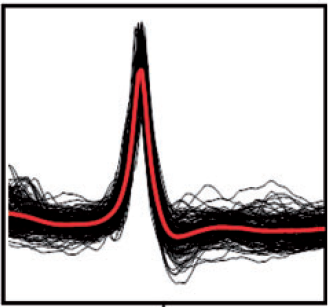
\includegraphics{text/SpikePatterFromStudie.png}
    \caption{Pattern of a spike derived from averaging 10-20 spikes in Boston et al \cite{MatchingFilter}}
    \label{fig:Patternstudie}
\end{figure}

Due to the difficulty in identifying this behavior without excellent filtering and neuroscientist's input, a spike has been loosely defined in this paper, the same as the one described in Seddik et al \cite{SpikeDetection}. A spike will therefore be described as when the EEG signal exceeds the value $100$mv for a duration between $20$ and $70$ ms.\\
\\
The two main approaches to identify these signal spikes are proposed in this paper, these are simple if statement or a more complex matching filter. The spike detection approach was of interest due to its low computational requirement, which was a potential problem that the hardware group foresaw. It requires no FFT and is a purely time-based analysis. It is also straightforward to implement on the MCU since it consists of basic programming principles such as for loops and if statements. Due to this, the method was explored as an alternative to more complex methods such as CNN. 



\subsubsection{Convolutional neural network}

A convolutional neural network (CNN) is a neural network structure that is frequently used in image-processing applications. They are known to be powerful, efficient, and easy to train, as long as you have a good dataset. The idea behind using them for EEG signals came from a paper \cite{CNNpaper}. Implementing a vanilla CNN is fiddly but straightforward, meanwhile getting a good dataset for it to train on is hard. \\

%(If necessary, maybe I can write a bit about setting up a vanilla CNN?)

A CNN uses kernels that go over an image, basically collecting information over a region, then summing it up and creating a new image. Each pixel in the new image contains information over a region the size of the kernel, but that data also overlaps between neighboring pixels since a data point in the original image may have multiple kernels run over them. \\

This can be done in multiple steps and in parallel with each other, having multiple kernels doing the same operation and creating multiple output images. The data is then usually pooled and flattened to be put into a regular forward-fed fully connected neural network. \\

In our case we are using two multi-channeled convolutional layers with leaky ReLU as the activation function, max pooled 2x2 then followed by a hidden layer with leaky ReLU, and then an output layer outputting to 3 neurons. The 3 output neurons represent the 3 potential states we are trying to differentiate between. The network could be considered a vanilla CNN. \\

Even though setting up a CNN can be complicated, using libraries such as PyTorch or similar alternatives makes the process quite straightforward. As is usually the case when dealing with Python, simply follow the generic structure of an example, and adapt it to fit your specific needs. The high-level nature of this approach does, however mean that one loses a lot of low-level control, and debugging something that ``should work" quickly becomes an unforgiving task. In our case, we had to redo the base code multiple times to get it to run properly. The problems usually originated from a misunderstanding of the Python syntax, or by using outdated components of poorly maintained libraries.

\subsection{Preprocessing}
Filtering measured EEG signals with digital filters and the removal of artifacts. 
\subsubsection{Digital filters}
Cascaded Integrator-Comb (CIC) Filters is a computationally efficient anti-aliasing filter that is suitable before performing a sample rate reduction (decimation). Also, CIC decimation filters can improve analog to digital resolution by oversampling the input.

\begin{figure}[H]
    \centering
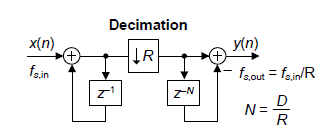
\includegraphics[width=0.35\textheight]{images/cic.png}
    \caption{Reduced comb delay, single-stage, CIC filter implementations for decimation \cite{CICguide}.}
    \label{fig:cic}
\end{figure}

Usually, a flat pass passband gain is desired where a Finite Impulse Response (FIR) filter can be used to compensate CIC's drooping gains \cite{CICguide}.

\begin{figure}[H]
    \centering
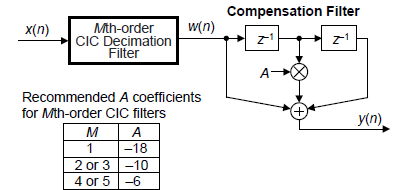
\includegraphics[width=0.35\textheight]{images/compFIR.png}
    \caption{A three-tap FIR compensation filter connected to an Mth-order CIC filter \cite{CICguide}.}
    \label{fig:cicfir}
\end{figure}

If the signal should not change in any way it can not be decimated but to not be left with no filtering at all a low-pass Fir filter can be implemented. Low-pass since the desired frequencies are in the 100 Hz and lower range.

\subsection{Artifact removal}
With the widely used electroencephalogram (EEG), brain activity can be measured and analyzed. However, due to its temporal and multi-source (non-invasive electrodes, here a set of 16) implementation, it is highly susceptible to artifact contamination. Artifacts may arise from measurement instruments and human subjects whereas physiological artifacts are more complicated to remove \cite{artifacts}. Instrument artifacts are removed by precise measurements and filters that were done by hardware and digital filters. With that, continuing, artifacts will aim at physiological artifacts such as eye movements, eye blinks, cardiac activity and muscle activity \cite{artifacts}. Below there are three examples of how such artifacts can look like.

\begin{figure}[H]
    \centering
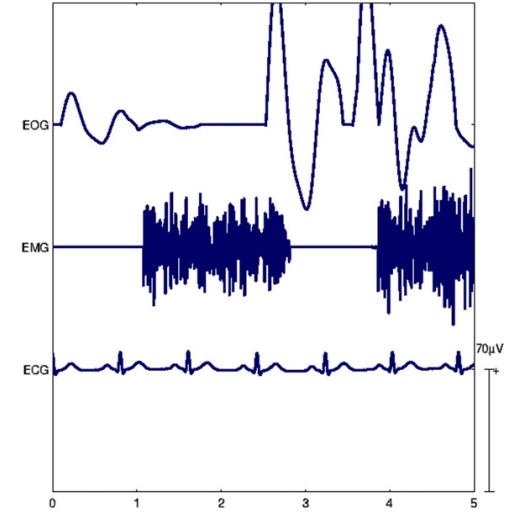
\includegraphics[width=0.35\textheight]{images/artifacts_image.png}
    \caption{\textit{Three different kinds of artifacts}. Ocular, muscular, and cardiac artifacts are the most frequent physiological contaminants. Source: Journal of Engineering no. 12 \cite{artifactsImage}.}
    \label{fig:artifacts}
\end{figure}

The most common approach to removing these artifacts is through ICA (Artifact removal of Independent Components) \cite{artifacts}. ICA is particularly good at identifying muscle artifacts (such as eye blinks) and is a widely-used blind source separation technique \cite{ICA}. There are several different ICA algorithms where the fastICA algorithm was chosen because of its speed (cubic convergence speed) and relative simplicity (few adjustable parameters). FastICA extracts components by maximizing the non-Gaussianity using fixed-point iteration \cite{ICA}. These extracted components, once analyzed, can then be classified as artifacts and subsequently removed.

This paper will not go into detail about the exact mathematical machinery of fastICA but what's important is to be familiar with these five matrices and one parameter:
\begin{itemize}
\item \textbf{X} - pre-processed data matrix [rows, cols]
\item \textbf{compc} - number of components to be extracted
\item \textbf{K} - a pre-whitening matrix that projects data onto the first compc principal components
\item \textbf{W} - estimated un-mixing matrix
\item \textbf{A} - estimated un-mixing matrix
\item \textbf{S} - estimated source matrix
\end{itemize}
W is the estimated un-mixing matrix and also where the estimated components can be found. It is this matrix (and its pseudo-inverse A) that needs to be analyzed for artifact behavior. In other words, ICA finds the constant matrix W from the relation $s=Wx$ and when this weight matrix is found by iteration and its component behavior subsequently analyzed, an output signal can be found by $x=As$ that contains less physiological contamination.


%\subsubsection{Dataset}

%\subsubsection{Feature extraction}

%\subsubsection{Prediction algorithm}
% Måste inte ha egen rubrik utan kan ingå i teorins löpande text.
% I fall teorikapitlet utelämnas ska litteraturstudie ingå i inledningen.
